\documentclass[10pt,a4paper]{article}    
\pagestyle{headings}
\usepackage{amssymb}
\usepackage{algorithm}
\usepackage{algorithmic}
\usepackage{graphicx}
\usepackage[margin=0.2in]{geometry}
\usepackage{cite}
\begin{document} 
\textsc{\\ \\ \\ \\ \centerline{\LARGE cs251--assignment 3} \\ \\ \centerline{\large Document on \LaTeX}}\\[1.5cm]
\hrule
{\vspace{1cm} \huge \bfseries Algorithm for long integer multiplication  \vspace{1cm}}


\hrule

\vspace{2cm}

\textsc{\Large Author:}

\textsc{\Large Gorank Dudeja(11283)}

\textsc{\Large G4}
\title{\huge Algorithm for Long Integer Multiplication}
\maketitle
\vspace{3cm}
\textsc{\centerline{\LARGE TABLE OF CONTENTS}}
\vspace{2cm}
\tableofcontents
\newpage

\section{Explanation of the algorithm}
\large This algorithm is really very simple.The main points are listed below
\begin{itemize}
\item Let us suppose we have to multiply a and b where both a and b are integers.\\
\item Let the smaller one of them be a and so a is multiplier and b is multiplicand. \\
\item First copy a and b into two other variables,say m and n. 
\item Divide m and n into its digits considering the units place,tens place,hundreds place and so on.\\
for example :- 324=300+20+4
\item Now,multiply both the digits of m and n taking into account the corresponding factors of 10\\
 and then add up all the products to get the result.
\end{itemize}

\newpage

\vspace{4cm}
\section{Pseudocode}
\begin{algorithm}
\begin{algorithmic}
\large
\STATE Let a be the multiplier and b be the multiplier.
\STATE Let factora and factorb be the factor of multiplication for a andb respectively 
\STATE Let rema be the last digit in a and remb be the last digit in b
\STATE factora=1,factorb=1,result=0
\STATE $ m \leftarrow a$
\STATE $n \leftarrow b$
\WHILE{1}
\STATE $rema \leftarrow m \% 10$
\WHILE {1}
\STATE   $remb \leftarrow n\%10$
\STATE  $result \leftarrow$ result+(rema*remb*factora*factorb)
\STATE  $n \leftarrow n/10$
\IF{$n == 0$}
\STATE $n \leftarrow b$
\STATE break
\ENDIF
\ENDWHILE
\STATE $ m \leftarrow m/10 $
\STATE $factora \leftarrow factora*10$
\STATE $factorb \leftarrow factorb*10$
\IF {$m ==0$}
\STATE  $m \leftarrow b$
\STATE break
\ENDIF
\ENDWHILE
\end{algorithmic}
\end{algorithm}
\newpage

\newpage
\section{Flowchart}

\begin{figure}
\centering
\caption{ Flowchart to illustrate the steps of the algorithm}
\label{flow:flowchart}
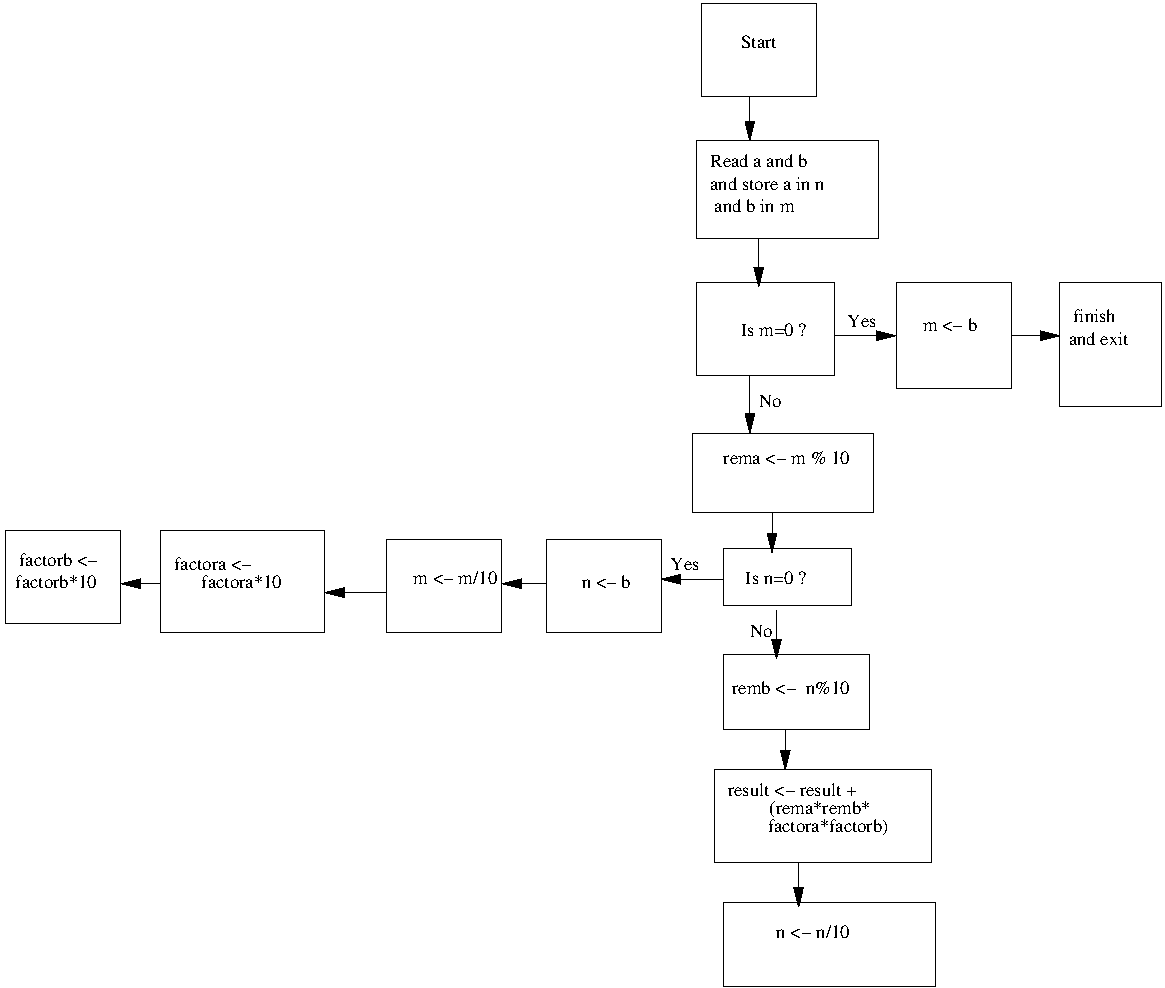
\includegraphics{flowchart}
\end{figure}

\newpage
\section{Example to illustrate the algorithm}

\begin{figure}
\centering
\caption{Example of multiplication of two integers}
\label{ex:example}

  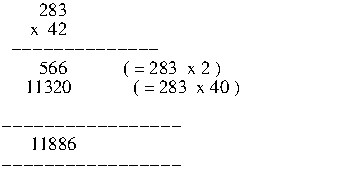
\includegraphics[scale=2]{example}
\end{figure}

\newpage
\section{Analysis of time complexity}
\large This algorithm has \textbf{\underline{two loops}} which are nested into each other.
\\
\\
The worst case that will be faced by the algorithm is when both the loops run upto n times where n is the number of digits in the
two numbers.
\\
\\
Some other operations are also executed in the algorithm like modulus operator,initialisation etc.
\\
 but they all take constant time and so, the worst number of instructions executed by the algorithm
is proportional to $n^2$ +k where k is a constant.
\\
\\
And so, the time complexity of the algorithm is O($n^2$) where O stands for Big-O notation.
\end{document}